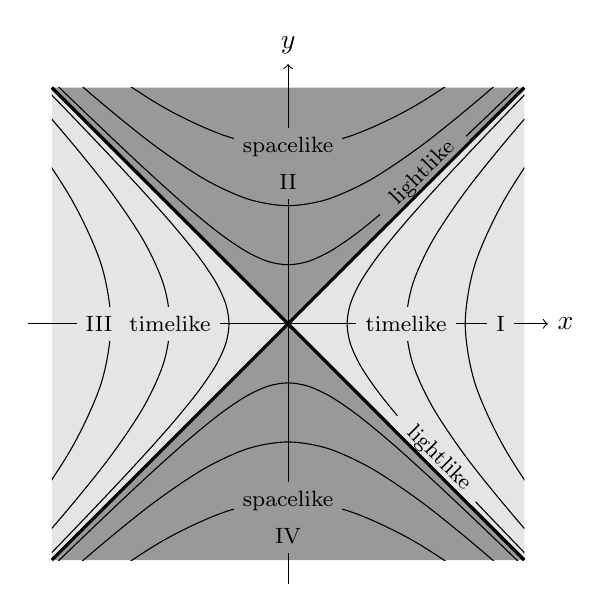
\begin{tikzpicture}[scale=1.5]
    
    \fill[fill=gray!20] (0,0) -- (2, 2) -- (2, -2) --cycle;
    \fill[fill=gray!20] (0,0) -- (-2, 2) -- (-2, -2) --cycle;
    
    \fill[fill=gray!80] (0,0) -- (-2, 2) -- (2, 2) --cycle;
    \fill[fill=gray!80] (0,0) -- (-2, -2) -- (2, -2) --cycle;
    
    \begin{scope}

        \clip (-2, -2) rectangle (2, 2);
        \foreach \K in {0.5, 1, 1.5} {
            \draw[smooth, domain=-4:4, variable=\t] plot ({\K*cosh(\t)}, {\K*sinh(\t)});
            \draw[smooth, domain=-4:4, variable=\t] plot ({-\K*cosh(\t)}, {-\K*sinh(\t)});
            
            \draw[smooth, domain=-4:4, variable=\t] plot ({\K*sinh(\t)}, {\K*cosh(\t)});
            \draw[smooth, domain=-4:4, variable=\t] plot ({-\K*sinh(\t)}, {-\K*cosh(\t)});
        }
    \end{scope}
    
    \draw[very thick] (-2, -2) -- (2, 2) node[above,pos=0.8, sloped,fill=gray!80,inner sep=0cm] { \ \rotatebox[origin=c]{90}{$\Lsh$} \footnotesize{lightlike} \rotatebox[origin=c]{270}{$\Rsh$} \ };
    \draw[very thick] (2, -2) -- (-2, 2) node[above,pos=0.2, sloped,fill=gray!20,inner sep=0cm] { \ \rotatebox[origin=c]{90}{$\Lsh$} \footnotesize{lightlike} \rotatebox[origin=c]{270}{$\Rsh$} \ };
    
    \draw[->] (-2.2, 0) -- (2.2, 0) node[right] {$x$};
    \draw[->] (0, -2.2) -- (0, 2.2) node[above] {$y$};
    
    
    
    \node[fill=gray!80] at (0, 1.5) {\footnotesize{spacelike}};
    \node[fill=gray!80] at (0, 1.2) {\footnotesize{II}};
    \node[fill=gray!80] at (0, -1.5) {\footnotesize{spacelike}};
    \node[fill=gray!80] at (0, -1.8) {\footnotesize{IV}};
    fill=w
    \node[fill=gray!20] at (1, 0) {\footnotesize{timelike}};
    \node[fill=gray!20] at (1.8, 0) {\footnotesize{I}};
    \node[fill=gray!20] at (-1, 0) {\footnotesize{timelike}};
    \node[fill=gray!20] at (-1.6, 0) {\footnotesize{III}};
                
    % TODO: Add some hyperbolas
    
\end{tikzpicture}